% source-figure:q18-solid, fixed science PDF p.1 / printed 961.
% Layout projection only; hidden AF changes style at its visible EC crossing.
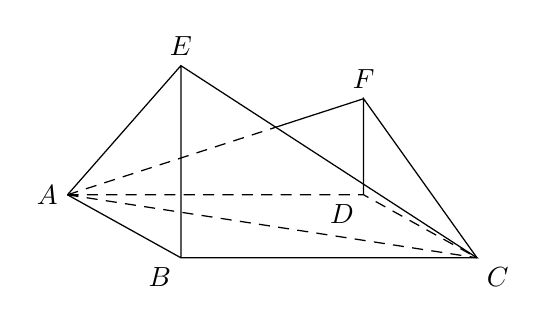
\begin{tikzpicture}[line width=.45pt,scale=.8]
  \coordinate (A) at (0,1);
  \coordinate (B) at (1.8,0);
  \coordinate (C) at (6.5,0);
  \coordinate (D) at (4.7,1);
  \coordinate (E) at (1.8,3.05);
  \coordinate (F) at (4.7,2.525);
  \coordinate (J) at (3.307,2.073);
  \draw (A) -- (B) -- (C) -- (E) -- (A) (E) -- (B);
  \draw (D) -- (F) -- (C) (J) -- (F);
  \draw[dash pattern=on 4pt off 3pt] (A) -- (J) (A) -- (D) -- (C) (A) -- (C);
  \node[left] at (A) {$A$};
  \node[below left] at (B) {$B$};
  \node[below right] at (C) {$C$};
  \node[below left] at (D) {$D$};
  \node[above] at (E) {$E$};
  \node[above] at (F) {$F$};
\end{tikzpicture}
